\documentclass[conference,final]{IEEEtran}
\usepackage{graphicx}
\usepackage{fixltx2e}
\usepackage{array}

\begin{document}
\title{Evolutionary Design of Self-Organizing Particle Systems for Collective Problem Solving}
\author{\IEEEauthorblockN{Benjamin Bengfort, Philip Y. Kim, Kevin Harrison, and James A. Reggia}
\IEEEauthorblockA{Department of Computer Science\\
University of Maryland, College Park, MD, USA\\
\{bengfort,reggia\}@cs.umd.edu, \{philip.y.kim,kharriso\}@gmail.com}}

\IEEEcompsoctitleabstractindextext{%
\begin{abstract}
Using only simple rules for local interactions, groups of agents can form self-organizing super-organisms or “flocks” that show global emergent behavior. When agents are also extended with memory and goals the resulting flock not only demonstrates emergent behavior, but also collective intelligence: the ability for the group to solve problems that might be beyond the ability of the individual alone. Until now, research has focused on the improvement of particle design for global behavior; however, techniques for human-designed particles are task-specific. In this paper we will demonstrate that evolutionary computing techniques can be applied to design particles, not only to optimize the parameters for movement but also the structure of controlling finite state machines that enable collective intelligence. The evolved design not only exhibits emergent, self-organizing behavior but also significantly outperforms a human design in a specific problem domain. The strategy of the evolved design may be very different from what is intuitive to humans and perhaps reflects more accurately how nature designs systems for problem solving. Furthermore, evolutionary design of particles for collective intelligence is more flexible and able to target a wider array of problems either individually or as a whole. 
\end{abstract}}

% make the title area
\maketitle

\IEEEdisplaynotcompsoctitleabstractindextext

\section{Introduction}

Flocks or swarms can be easily simulated by creating individual agents whose motion is determined solely by local interactions with their neighbors. Although the individual agent can only see those neighbors closest to it, self-organizing movement of a population composed of many of these simple agents will emerge - the flock or swarm. This property of collective behavior was first demonstrated by Reynolds \cite{reynolds1987flocks} who was attempting to simulate the behavior of flocks of birds as multi-agent systems particularly for animation. Since then, there has been interest in extending such systems to solve more general problems. The self-organizing characteristic of these systems, whereby coordinated behavior emerges without a central control mechanism, suggests that even relatively simple decentralized systems might yield novel approaches to problems in both the computational and physical domains.

For example, by abstracting the idea of ``flocks'' to $n$-dimensional spaces, particle swarms \cite{kennedy1995particle,clerc2002particle} and cultural algorithms \cite{chung1996testbed} have been used for numerical optimization. In the physical domain, swarm behaviors have been used to control multi-robot team movement \cite{balch1998behavior,ccelikkanat2010steering,hodgins1994robot}, and the deployment of mobile robots or sensors. In \cite{cheng2009distributed}, flocking behavior was used to maximize area coverage during such deployments by coordinating movements via collective behavior. Other tasks being explored use collective problem solving for a variety of tasks including urban pursuit \cite{winder2004using}, where a team of agents moves through an obstructed landscape to catch a target that moves faster than each individual in the chase team. Although these domains are very different, from optimization to herding, all rely on the principle of emergent flocking behavior of individuals following only local rules.

In order to achieve collective problem solving beyond simple flocking movement, additional local behaviors besides individual motion are required. Many approaches augment flocking agents with additional features that still rely only upon local context, but in aggregate, demonstrate an emergent, global behavior. For example in \cite{winder2012role,hu2003particle}, agents and particles were augmented with a short-term working memory that led to more efficient navigation of the entire flock and to better performance of numerical optimization. This paper in particular builds upon the work of Rodriguez \& Reggia in \cite{rodriguez2004extending}, who added both working memory and a finite state machine (FSM) controller that switched the agent between different sets of movement behaviors according to its local environment and current goal. They were able to demonstrate that a team of such agents was able to solve a resource locate-and-collect problem, and that a team programmed with flocking behaviors outperformed teams of agents that did not influence each other's movements.

Attempts have been made to formalize the design of such cooperative multi-agent systems \cite{mataric1993designing,capera2003amas}. In this paper, however, we turn to evolutionary computation techniques. Genetic Programming (GP) \cite{koza1992genetic}, Evolutionary Strategies \cite{rechenberg1989evolution}, and Genetic Algorithms \cite{goldberg1988genetic} have demonstrated the potential of computational design techniques for machine learning, optimization, and even engineering. Swarm techniques have even been applied to evolutionary computation itself as in  \cite{wei2002swarm,miranda2005evolutionary}. However, we are more interested in the reverse application, using evolutionary techniques to create particles that exhibit swarm behavior and collective problem solving. Because finite state machines have been evolved to solve problems such as automatic target detection \cite{benson2000evolving}, evolving the high level controllers of individual particles to produce collective behavior seems like an extension of the design of multi-agent problem-solving that is inspired by natural design. 

In this paper, we will show improvements upon the human design of particles, particularly those described in \cite{rodriguez2004extending}, by applying evolutionary techniques to the agent control mechanisms that lead to emergent problem solving. A formal human design technique determines the structure of the FSM and the parameters defining each state through empirical techniques and inspection. In contrast, we begin with a population of randomly-generated FSM configurations, run them through a simulated problem, then evolve the population over many generations through fitness-based selection, recombination, and mutation. Our hypothesis is that the resulting FSM configuration will perform as well as or better at a particular task (search and retrieve) than a configuration tuned by a human.

The paper is organized as follows: in the first section we will describe the methodology of our work in phases. The first phase will be to describe the particular problem domain that we evolved our flocks for - a locate and collect task. We will then describe how the movement behaviors of the flocks were defined and parameterized in terms of velocity computation and a controlling FSM. In the last phase we will discuss how we evolved each flock given the particulars of our simulation. Finally the methodology of our experimental procedure will be discussed, along with results and a concluding discussion.

\section{Methodology}

In order to best demonstrate that an evolutionary process can generate an agent controller that is competitive with a human designed one, we have created an experimental setup that is intentionally similar to the work done in \cite{rodriguez2004extending} and we have done our best to reproduce as exactly as possible the experiment and task as described in that paper. By recreating a specific collective intelligence task, we hope to directly compare a human designed particle system to an evolution designed one. 

\subsection{A Locate and Collect Task}

The task is a simulated multi-agent swarm (MAS) environment that is applicable to many modern day problems: a team of simulated agents starting from a particular location must locate and collect resources that are spread across a large two-dimensional world with periodic boundary conditions, then return the resources to a designated home base. Problem solving in this task involves a balance between exploring the world space for resources and exploiting already discovered resource deposits.

The individuals of the team operate as a flock: local rules determine individual movement and individual goals lead to emergent collective behavior. Each individual has a limited sight range and angle, the ability to communicate with other, nearby agents and a limited working memory. Particle behavior is governed by a finite state machine that determines how each particle moves given its individual state and the environment around it.

The task is competitive as there are two teams in the environment competing for resources. Each team has different traits exhibited by their movement behaviors and also random starting locations within a certain distance from their home base. Because of these two factors, how each flock initially behaves is based on the random assignment of their positions. Moreover, this assignment also determines how each flock behaves when encountering the opposing team. Agents can mine resources not only from designated depots, but also steal from the home base of the other team. The winner of a simulation is determined as the team that has the most resources in their home base at the end of a predetermined number of time steps. No two simulations will run exactly the same way therefore the simulation is non-deterministic.

Our evolutionary process uses this simulation to pit individuals created via genetic operations against the best designed human agent. The fitness of the evolved team is a function of the resources that they have collected versus the resources the other team collected against them. The next generation of evolution is then dependent on the fitness of teams as run in the simulation. In the parlance of evolutionary computing, the genotype is the real valued vector that represents the finite state machine of the particle and the phenotype is the emergent behavior of the team as a whole as it participates in the simulation.

In this section we will present the details of the simulation, as well as the details of the evolutionary computation mechanism that searches for the optimal, most economic particle in the simulation.

\subsection{Simulation}

\begin{figure}[t!]
    \centering
        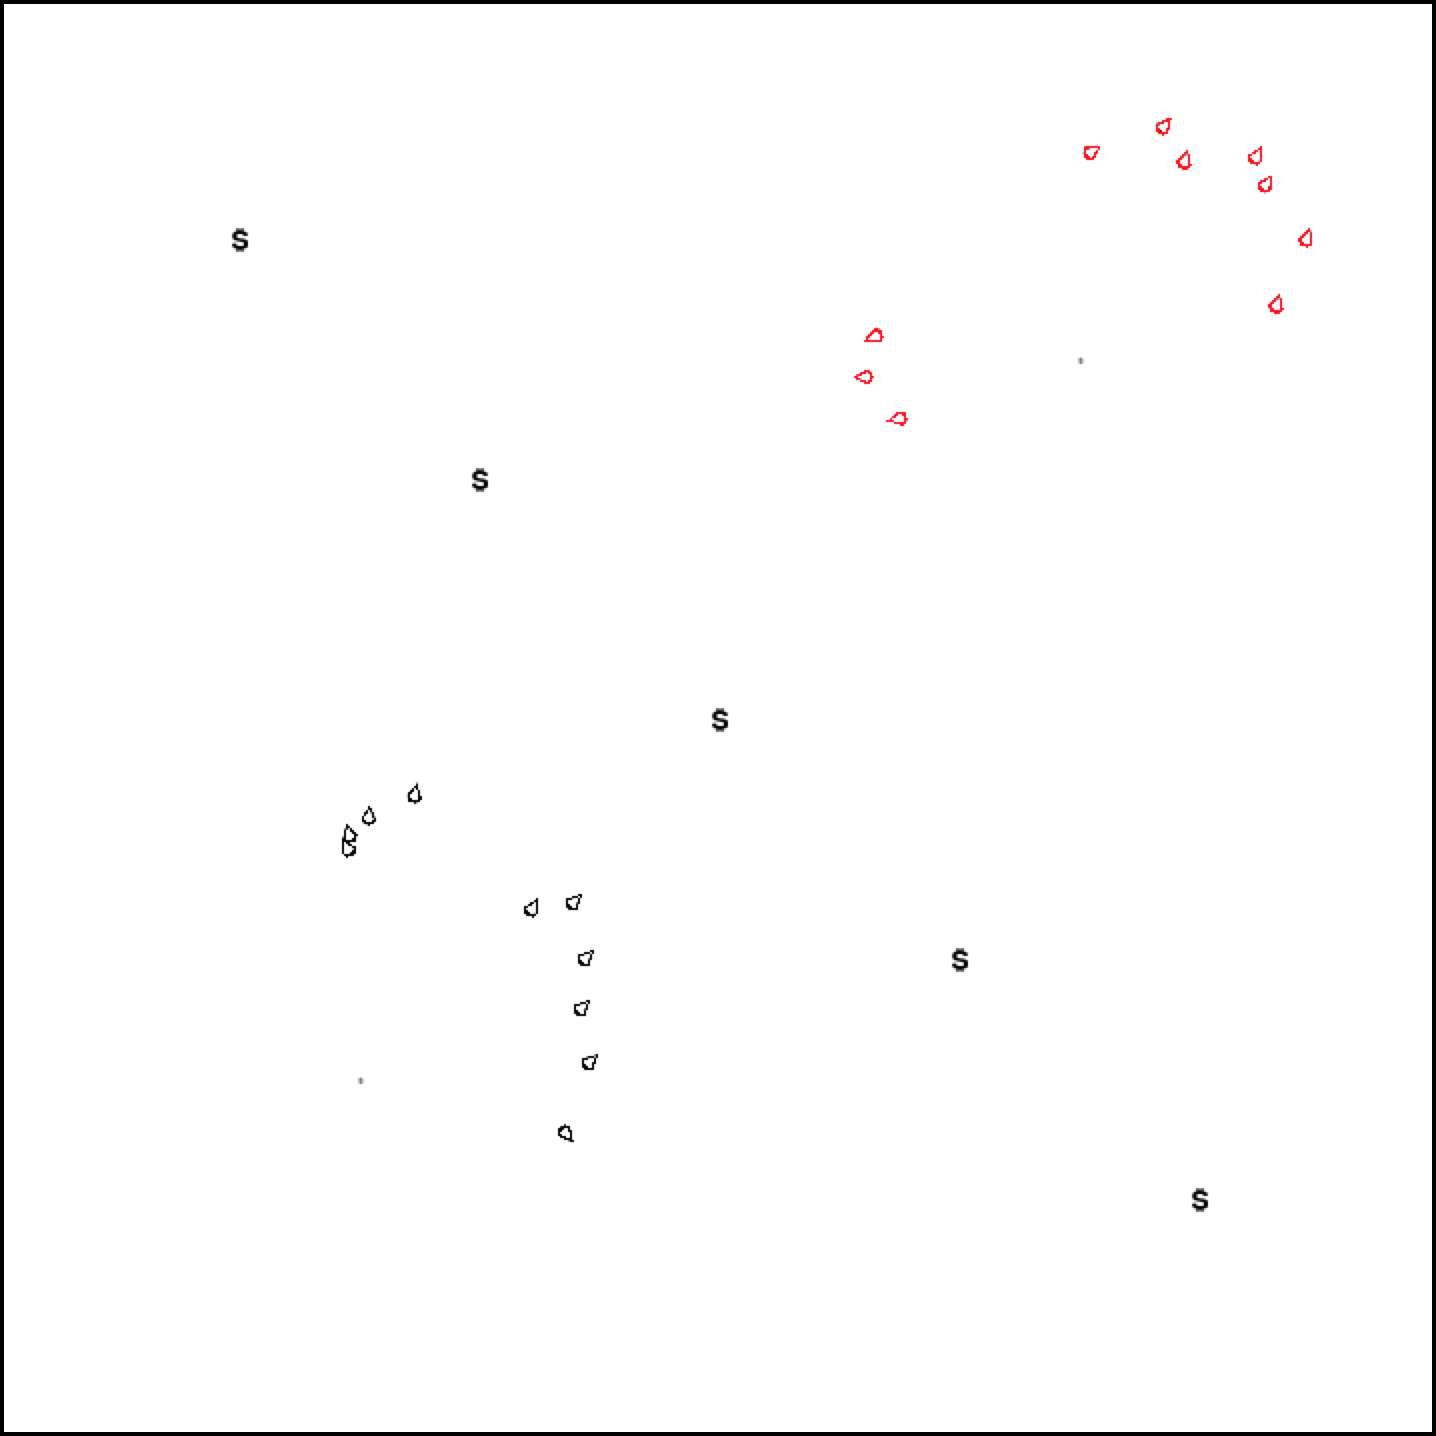
\includegraphics[width=0.5\textwidth]{figures/simulation}
    \caption{Screenshot of visual simulation showing agents spreading in flocks. This figure shows two teams moving with flocking behavior; a black team and a red team separated by resources shown as dollar signs.}
    \label{fig:simulation}
\end{figure}

The movement behavior of individual particles is governed by local interactions of relatively close by particles within a particular neighborhood. Each particle updates its velocity at each timestep based on what it observes in the world around it and its current state. This leads to self-organizing, emergent behavior of the flock as a combined whole of its individuals. In particular, movement behaviors are updated via six possible velocity components: cohesion, alignment, separation, seeking, clearance, and avoidance. Together these components enable flocking behavior and minimize collisions. Figure \ref{fig:simulation} demonstrates this flocking behavior, as well as provides a visual description of the world; in it two teams, one at each of the bottom left and top right corners, are flocking to explore the world to find and exploit resource deposits, represented as dollar signs in our simulation.

Collective problem solving emerges by equipping individual particles with an FSM controller that determines specific goals of the particles, along with a limited working memory. Each state is a combination of a goal, for example SEEKING, as well as a set of state-specific parameterized velocity components that determine the movement behavior of a particle in that state. Transitions between states occur due to local observations of the world in a particle's limited sight distance- for example, if a particle detects a resource in its neighborhood, it will switch to the HOMING state to move more directly toward the resource, which will also have the effect of pulling along particles that have not observed the resource. In each state, the particle still exhibits flocking behavior, but the swarm as a whole can have individuals in multiple states to strike a balance between the exploration of the world and the exploitation of discovered minerals.

Some real world constraints are also placed on the particles. For example, if particles from opposing teams collide, they are both frozen. In the human designed particle swarm, this condition allowed for the creation of GUARDING states. In the next sections we will describe the velocity components and associated movement behaviors.

\subsubsection{Velocity Components}

It is important to discuss each individual velocity component in detail, as these components define the aggregate movement behaviors of states that compose an FSM controller that is being evolved. Every component has several parameters: a radius, $r$, and alpha, $\alpha$, which determine the sight distance and angle of the neighborhood of the particular component. Each component additionally has a weight, $w$, which is used to determine the contribution of the component to the final velocity of the particle.

All particles are bound by a maximum velocity, $v_{max}$, and for the purposes of evolution, a maximum radius, $r_{max}$, to simulate economic constraints in the world. Other notation used is as follows: $\Delta \vec {p} = \vec {p_n} - \vec {p}$, where $\vec {p_n}$ is the average of the neighbor positions and $\vec p$ is the position of the agent. Similarly $\Delta \vec {v} = \vec {v_n} - \vec v$, where $\vec {v_n}$ is the average of the neighbor velocities and $\vec v$ is the velocity of the agent. Other positions include $\vec p_e$ which is the position of an enemy agent, and $\vec p_t$, the position of a target. $\vec p_\perp$ represents a unit vector orthogonal to the agent in the $+z$ direction. Specific velocity components are defined as follows.

\textit{Cohesion} (\ref{eqn:cohesion}): a vector pointing towards the average position of friendly agents in the neighborhood, with a magnitude proportional to the agent's distance to the center of its neighbors. This component increases quadratically with distance until it is equal to the maximum velocity when the distance to the neighbor center is $r$. The neighborhood includes all team members who are not guarding or stunned. This velocity component ensures that flocks form and stay together throughout movement.

\begin{equation}
    \vec { v_{ c } } =v_{ max }\frac { \Delta  \vec { p }  }{ \left\|   \Delta \vec { p }  \right\|  } \left( \frac { \left\|  \Delta \vec {  p }  \right\|  }{ r }  \right) ^{ 2 }
    \label{eqn:cohesion}
\end{equation}

\textit{Alignment} (\ref{eqn:alignment}): a vector in the same direction as the average velocity of friendly agents in the neighborhood, with magnitude proportional to the agent's distance to the center of its neighbors. This component increases quadratically with distance until it is equal to the maximum velocity when the distance neighbor center is $r$. The neighborhood includes all team members if they are seeking or spreading. Alignment helps the flock travel in the same direction in a coordinated fashion.

\begin{equation}
    \vec { v_{ al } } =v_{ max }{\left( \frac { \left\| \Delta \vec { p } \right\|  }{ r }  \right)}^2\frac {\Delta \vec{v}} { \left\| \Delta \vec{v} \right\| }
    \label{eqn:alignment}
\end{equation}

\textit{Separation} (\ref{eqn:separation}): a vector pointing away from the average position of friendly agents in the neighborhood, with magnitude inversely proportional to the distance from the agent to the center of its neighbors. This component decreases quadratically with distance until it is zero when the distance to the neighbor center is $r$. The nighborhood includes all team members no matter their state. Separation prevents particles in the same team from colliding with each other, as well as distributing the flock outwards.

\begin{equation}
    \vec { v_{ d } } =-v_{ max }\frac {\Delta \vec{p}} { \left\| \Delta \vec{p} \right\| }{\left( \frac { r - \left\| \Delta \vec { p } \right\|  }{ r }  \right)}^2
    \label{eqn:separation}
\end{equation}

\textit{Seeking, Homing, and Mineral Cohesion} (\ref{eqn:seeking}): vectors pointing directly towards a target with a magnitude proportional to the maximum velocity. These velocity components allow the particle to navigate in a  meaningful manner. The target is stored in memory and this velocity component isn't influenced by nearby neighbors.

\begin{equation}
    \vec{v_h} = v_{max} \frac {\vec{p_t} - \vec p} { \left\| \vec{p_t} - \vec p \right\| }
    \label{eqn:seeking}
\end{equation}

\textit{Clearance} (\ref{eqn:clearance}): a vector pointing in a direction orthogonal to the difference between the average neighbor position and the agent's position proportional the the maximum velocity. This component ensures that swarms have a wide field of view by spreading the flock laterally along the front of movement. The neighborhood of this component is team members in sight that are not guarding or stunned.

\begin{equation}
    \vec{v_{cl}} = v_{max} \frac {\Delta \vec p_\perp } { \left\| \Delta \vec p_\perp  \right\| }
    \label{eqn:clearance}
\end{equation}

\textit{Avoidance} (\ref{eqn:avoidance}): a vector pointing away from an enemy agent in the neighborhood, with magnitude $v_{max}$, when distance to the enemy is zero and decreasing linearly with distance until it is zero when the distance is $r$. Unlike all the other components, this can be applied multiple times each timestep -- once for every enemy in the neighborhood.

\begin{equation}
    \vec { v_{ av } } =\sum _{i=0}^{n} {v_{ max } \left( \frac{r - \left\| \Delta \vec{p_e} \right\|} {r} \right) \frac { \Delta \vec { p_e }  }{ \left\| \Delta \vec { p_e }  \right\|  }}
    \label{eqn:avoidance}
\end{equation}

\subsubsection{Movement Behavior}

The FSM controlling each agent in our first experiment contained four states: searching for new resources (SPREADING), moving to the last known resource deposit (SEEKING), carrying resources back to the home location (CARAVANING), or guarding the home base or a resource deposit (GUARDING). Each state was composed of some combination of the previously described velocity components, specifically parameterized for each state.

To update the velocity of a particle at time $t$, a simple linear combination of velocity components was used. The components, along with their parameters and weights, depended on the current state of the particle. The magnitude (or length) of the vector was maximized at $v_{max}$ in the direction of the computed component velocity. Our simulation also implemented ``inertia'', whereby the velocity was not combined from zero but rather added to the velocity at time $t-1$ (\ref{eqn:velocity}). The position of the particle at time $t$ was simply the sum of the position at time $t-1$ with the new velocity (\ref{eqn:position}).

\begin{equation}
    \vec {v_t} =  \vec {v_{t-1}}+ \sum_i^c { w_i v_i}
    \label{eqn:velocity}
\end{equation}

\begin{equation}
    \vec {p_t} = \vec {p_{t-1}} + \vec {v_t}
    \label{eqn:position}
\end{equation}

Transitions between states were triggered by conditions in each agent's local environment according to rules governed by the FSM. For example, an agent in the searching state that detected a mineral deposit within a 200-unit radius (in any direction) would push that deposit onto the top of its memory stack and transition to the seeking state (which is characterized by movement toward the top location on its stack).

One of the main findings in \cite{rodriguez2004extending} was that it was advantageous for the agents to post "guards" on their homes and/or on any discovered resource deposits. Agents that guarded only the home performed best of all, though agents that guarded both the home and deposits still outperformed non-guarding agents. In order for guarding behavior to be feasible, however, agents must avoid agents on the enemy team. Since we were allowing evolution to determine the strength of this avoidance parameter, we expected that in the absence of an enforced motivation for avoidance, the avoidance parameter would be selected down to zero, allowing the agents to ignore enemy guards.

Therefore we implemented a penalty for colliding with another agent. An agent within 10 units of an enemy agent was rendered unable to move for a number of timesteps equal to 180 minus the angle of incidence in degrees. For example, if an agent collided with an opposing agent at right angles, the agent struck in the side would be unable to move for 90 timesteps, whereas the agent struck in the front would be unable to move for 180 timesteps. Similarly, being "rear-ended" by an opposing agent had no penalty at all. The hope was that by assigning the "responsible" agent more of the penalty, we would create an incentive to avoid collision.

In order to allow for the selection of guarding behavior, the transition to the guarding state was controlled by two  evolvable parameters -- the \textit{home guarding threshold} and the \textit{deposit guarding threshold} -- which specified the number of friendly agents considered sufficient to guard the respective sites. A value of 0 disabled guarding behavior. This is currently the only instance in our simulation where a transition between states was controlled by an evolvable parameter.

A single timestep in the world can be characterized as follows. Each agent is in a particular state. For each velocity component in its current state, it determines the number of friendly and enemy agents in the respective neighborhood and calculates the direction and magnitude of the component. These components are linearly summed, and the resulting velocity is subjected to the $v_{max}$ constraint. The agent's position is updated by adding the velocity to the agent's position in the previous timestep. The agent then determines whether it should change its state based on the predefined transition rules and its current environment. All agents make this computation simultaneously; updating does not affect the world in the current time step.

\subsection{Evolution}

\begin{table}[t!]
    \renewcommand{\arraystretch}{1.5}
    \centering
    \caption{Characterization of Evolutionary Method}
    \label{table:evolvemethod}
    \begin{tabular}{|l|l|}
        \hline
        Genotype & Real valued vectors representing FSM states \\
        Phenotype & Swarm behavior from individual movements \\
        Selection & Tournament with elitism \\
        Recombination & Intermediary exempting elites \\
        Mutation & Linear rule exempting elites \\
        Fitness & Resources collected after 10k timesteps \\
        Specialty & Adapting FSM with same size network \\
        \hline
    \end{tabular}
\end{table}

The evolution of a finite state machine for movement control was achieved through the application of a simple set of genetic operators to the states of the FSM as defined by a collection of velocity components and their behavior specific parameters. The genotype for our simulation was represented as a vector containing two integers, one for each guarding threshold, and real-valued numbers consisting of the alpha parameter, radius, and weight given to each component of each compound movement behavior.

In this experiment, the set of states in each controller was fixed to be the same set of compound behaviors as those found in \cite{rodriguez2004extending}, but with parameters derived through evolutionary programming. This allowed for easy comparison with the authoritative, human-derived solution. In addition, the transitions between states were kept the same except for the guarding thresholds, which were evolved. The basic evolutionary computation was a mixture of Evolutionary Strategy and Evolutionary Programming techniques as described in \cite{eiben2003introduction}. The implementation is characterized in Table \ref{table:evolvemethod}. 

The mutation operator first selected which parameters to modify independently. We used a mutation probability parameter $p_m=0.2$  for mutating each weight, radius, alpha, and threshold. Each selected threshold had an equal chance of increasing by 1 and decreasing by 1. Each selected real-valued parameter was modified through the addition of a uniformly distributed random number with mean 0. We mutated each weight with world constraints using $r\in\left(1,500\right]$ and $\alpha\in\left(0,360\right]$. The step size of the mutation was $m_w\in\left[-0.2,0.2\right]$ for weights and $m_s\in\left[20,20\right]$ for the $r$ and $\alpha$ parameters. Elite individuals were exempted from mutation.

The recombination operator also ignored the elite individuals carried over from the last population. Parents were selected with a recombination probability, $p_r=0.2$, to be recombined with another individual. We used intermediary recombination of the weight, radius, and alpha parameters of all components in all states, bounded by the minimum and maximum possible values of each parameter. The second chosen parent remained in the population. Although elite individuals were exempt from recombination, they were able to be selected as the secondary parent, contributing their genetic material to the recombined offspring.

A round of evolution consisted of the evaluation of the fitness of every individual followed by the application of elitism, tournament selection, recombination, and mutation to produce the next generation. For elitism, the $N_e$ individuals of the previous generation were always carried into the next generation without modification. The other $p-N_e$ individuals were selected via tournaments of size 3. All non-elite individuals chosen through the tournament then had a $p_r$ chance of undergoing recombination with another randomly chosen child. Each of the resulting non-elite individuals was then subjected to the mutation operator, mutating parameters independently, with a probability of mutation, $p_m$.

\section{Experimental Procedure}

Our computational experiment required two main components: a system to carry out the evolutionary computation, which constructed genotype populations via genetic operators, and a simulation system to instantiate phenotypes -- particle swarms whose individuals are constructed from the genotypes. The simulation system computed the fitness of a particular swarm, which allowed the evolutionary computation to build the next generation. The simulation process is computationally expensive, and as such limited our ability to conduct multiple evolutionary runs -- each evolution took at least a week to complete.

The simulation environment consisted of two simulated teams in competition with each other; a red team and a black team. The simulated world was represented as a two dimensional square grid with a height and width of 3000 units and periodic boundary conditions. The simulation clock incremented by one at each timestep and was limited to 10,000 ticks per simulation due to computational constraints. We restricted each team to 10 agents each, and evenly distributed 5 resource deposits between the red and black bases with 80 resources per deposit. The simulations were run on a headless server, but a visual demonstration of each simulation could be run; the state of the world and the starting locations of the swarms can be referred to in Figures \ref{fig:simulation} and \ref{fig:spreading}, which are screenshots of the visual simulations.

Both the team size and the time limit were implemented to make the evolutionary computation tractable; our implementation required on average 273 CPU seconds to complete a single simulation for fitness evaluation; and each generation took approximately 52 minutes to compute all fitness values running eight simulations in parallel. For an evolutionary process of 100 generations, this meant at least five days of continuous computation were required to complete a single experiment.

The red team's behavior was implemented using a finite state machine, memory, and movement parameters exactly as the best empirical result designed by humans in \cite{rodriguez2004extending}, called \textit{home guarding flock}, meaning that the swarm guarded its home base but not discovered mineral deposits. The black team utilized the configuration derived from a genotype individual produced by the evolutionary computation. We attempted to hold as many variables constant as possible, including the locations of bases and resources, starting positions and velocities of agents, and update order. After 10,000 timesteps, the fitness of the black team was returned as the number of resources in the black base.

The evolutionary process randomly initialized a population of 50 black team configurations, then ran a simulation for each individual in the population. After all 50 simulations were completed, tournament based selection with tournaments of size three were carried over to the next generation along with the five most elite individuals. After selection, genetic operators were applied to produce the next generation.

Because of the computational expense, we ran only two evolutionary experiments. In our first experiment we used only mutation to change the states in the finite state machine of the particles. In the second experiment we used recombination in addition to mutation operations. In either case, elite individuals were exempt from genetic operations, though elite individuals could be recombined to replace other individuals in the population. Both the mutation and recombination (when used) had a likelihood of 0.2. Maximum and minimum parameters were also placed on the values of the weight, the radii, and the alpha values to ensure an economic and reasonable result.

\section{Results}

\begin{table}[t!]
    \renewcommand{\arraystretch}{1.5}
    \centering
    \caption{Fitness of particles competing against human designed particle.}
    \label{table:meanfitness}
    \begin{tabular}{l | c c cc}
        \hline
        Simulation & Mean & Std Dev & Max & Min \\
        \hline
        human vs human & 249.125 & 42.618 & 319 & 177 \\
        evolved vs human & 397 & 4.833 & 400 & 386 \\
        \hline
    \end{tabular}
\end{table}

\begin{figure*}
\centering
\begin{minipage}{0.5\textwidth}
	\centering
    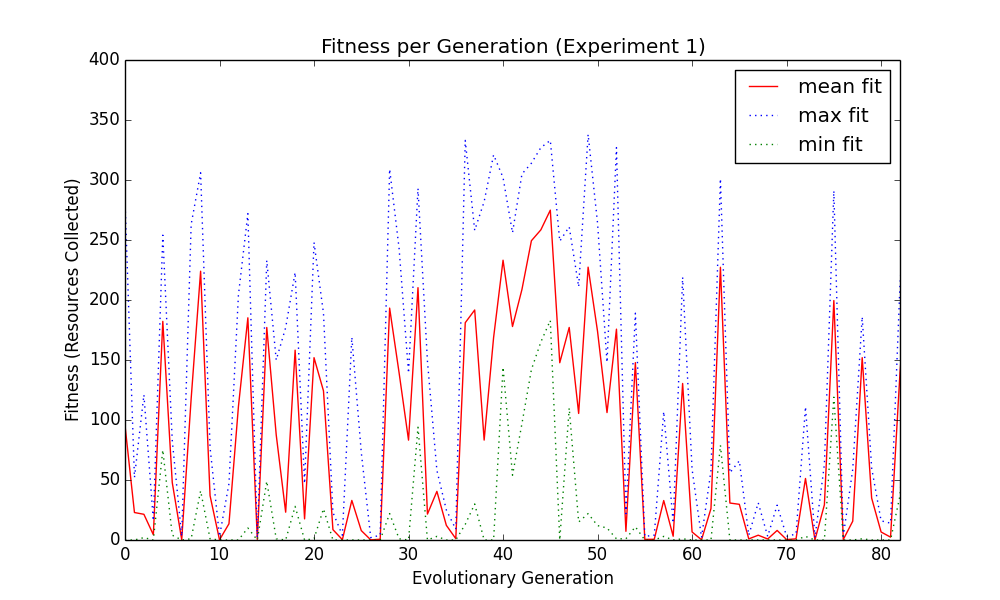
\includegraphics[width=\textwidth]{figures/meanfit_experiment1}
    \caption[width=0.45\textwidth]{Experiment 1 evolved swarms with mutation alone but did not \\ achieve convergence and was stopped after 82 generations.}
    \label{fig:meanfit1}
\end{minipage}%
\begin{minipage}{0.5\textwidth}
	\centering
    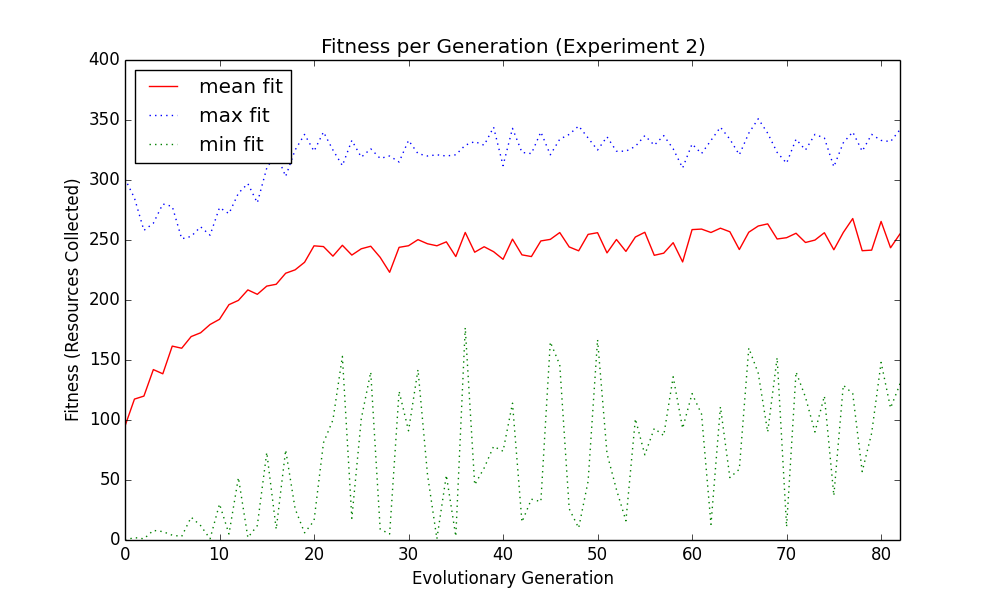
\includegraphics[width=\textwidth]{figures/meanfit_experiment2}
    \caption[width=0.45\textwidth]{Experiment 2 performed evolution with both mutation and recombination, convergence was achieved after approximately 50 generations.}
    \label{fig:meanfit2}
\end{minipage}
\end{figure*}

Evaluation of the evolutionary process to design a particle that could perform a collective intelligence task consisted of evaluating the evolutionary process to see if it converged and produced a particle that could compare to the human designed particle in the collect and locate task. We observed that the evolutionary computation mechanism was able to design a particle system that exhibited variations in behaviors that were different enough from the human designed particles so as not only be competitive with the human designed team, but able to defeat this team in terms of resources collected.


The performance of our two evolutionary processes is expressed in Figures \ref{fig:meanfit1} and \ref{fig:meanfit2}, which plots the mean, maximum, and minimum fitness of the entire population for each generation. In our first experiment (Fig. \ref{fig:meanfit1}), only the mutation operator was used to generate the next population. Unfortunately, the evolution was unstable in terms of its search across the optimal state space. This may have been due to the fact that highly variable mutation caused dramatic shifts in the behavior of the phenotype and that elite genotypes were not able to contribute their genetic material to the next generation.

Our second experiment (Fig. \ref{fig:meanfit2}) consisted of changing the evolutionary computation mechanism to ensure the search space was more consistent. Instead of including one elite in the next generation, we carried five elites over. We also revised our mutation operator to ensure that it was mutating in small, linear steps. Finally, we also implemented recombination to try to allow genetic material from elites to influence the entire population. 

The second experiment used 50 individuals per population and ran for 100 generations. The revised evolutionary algorithm converged after approximately 50 generations, demonstrated in Figure \ref{fig:meanfit2}. The individual with the maximum fitness across all generations was discovered in population 97, but the maximum fitness individuals were also very close and consistent after 50 generations. Not only was this a much better result than our first evolutionary computation experiment in terms of reaching a converging fitness with little variability in population performance, but also each generation exhibited different behavior than their parent generation.

To evaluate the performance of our evolved particle swarm, we compared the performance of both the evolved and human designed particles competing against a human designed particle, using the same human designed team competing against itself as a baseline. Both the human and evolution designed particles were run in the simulation 32 times against the baseline team. The performance at each timestep was computed as the mean resources in the home base of each team. Further, we extended the maximum timesteps for the simulation from 10,000 (the maximum timesteps used to determine fitness during the evolutionary process) to 20,000 to see if any different behavior resulted and to ensure that the swarms had enough time to collect all the resources. 

As illustrated in Table \ref{table:meanfitness}, the evolved swarm collected over 100 more resources on average than the human designed swarm, with a significantly lower standard deviation. Averaged across all timesteps, Figure \ref{fig:head2head1} shows the performance of the human designed versus human designed particles,while Figure \ref{fig:head2head2} shows the performance of evolution designed versus human designed swarms. Competing against each other, the human design swarms do equivalently in competition. However the evolution designed swarm is able not only to capture more resources faster, but around timestep 7000, begins to steal resources from the enemy base. 

\begin{figure*}
\centering
\begin{minipage}{0.5\textwidth}
	\centering
    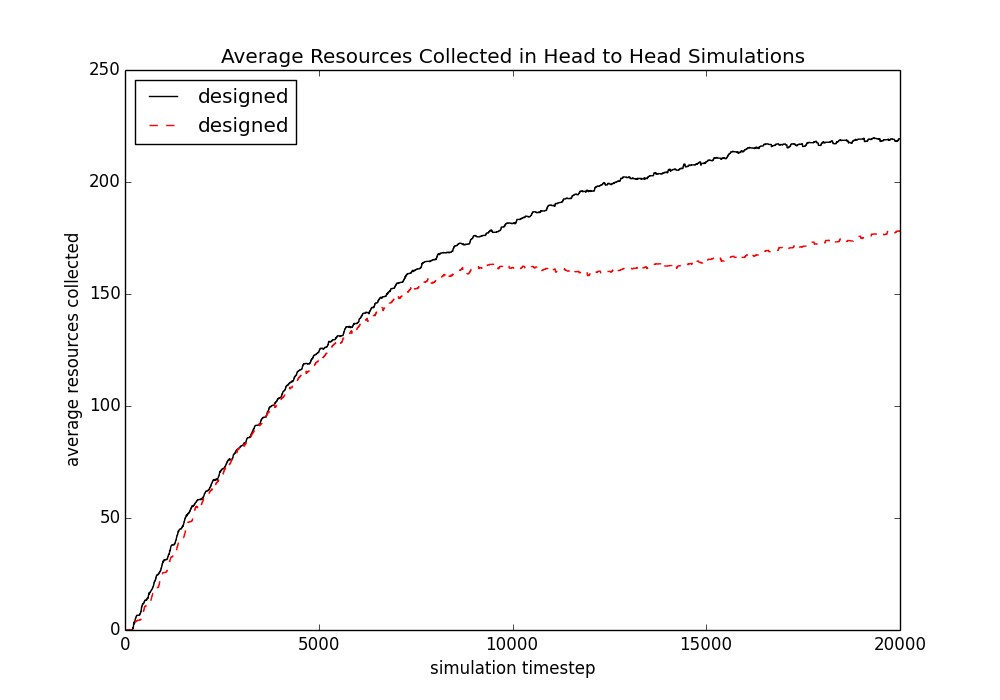
\includegraphics[width=\textwidth]{figures/designed_v_designed}
    \caption[width=0.45\textwidth]{The baseline was two identical human designed swarms compet- \\ ing against each other, resulting in similar performance collecting resources.}
    \label{fig:head2head1}
\end{minipage}%
\begin{minipage}{0.5\textwidth}
	\centering
    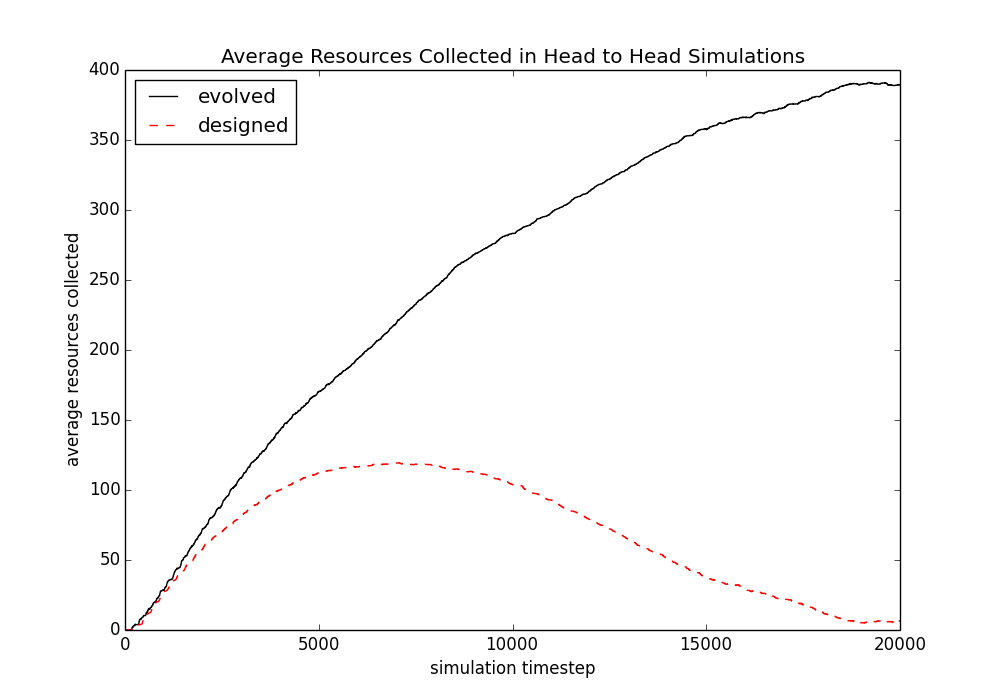
\includegraphics[width=\textwidth]{figures/evolved_v_designed}
    \caption[width=0.45\textwidth]{The evolved swarm was able to significantly outperform the human designed swarm and even managed to collect all resources.}
    \label{fig:head2head2}
\end{minipage}
\end{figure*}

From empirical observation of the best performing teams, it appears that the human designed team preferred to stay in one or two larger flocks, whereas the high performing evolved teams split into many smaller flocks and were able to exploit the search space more effectively. Because of the limited time frame in the simulation, this was clearly a better strategy, favoring early exploration and later exploitation of resources.

The evolved swarm also exhibits a very different spreading behavior than the human designed swarm. In Figure \ref{fig:spreading} the evolved particles spread more radially, able to explore more of the world earlier on. Another characterization of the differing behavior of each group is the size of the swarm, which is much larger, but then breaks apart into smaller swarms once resources are discovered, in order to better exploit more resources deposits at once. In contrast, the human designed particles tend to stay in one or two larger flocks and only exploit one depot at a time.

\section{Discussion}
A nature-inspired, evolutionary technique was successfully able to design particles that not only exhibited collective, emergent behavior, but also surpassed their human design counterparts by demonstrating significantly different behavior. For example, although guarding behavior was demonstrated as having a positive effect on resources collected in the human designed team, the best evolution designed teams did not implement a guarding movement behavior either for their home base or the mineral deposits, instead preferring a strategy of speed in exploration. Perhaps against a differently behaving team, the best evolution designed team would have evolved guarding behavior. In order to increase the variability of behavior, future work should include speciation as well as competitive co-evolution (evolving both teams simultaneously). This will hopefully lead to more general, adaptive designs that are not solely influenced by the environment in which they were evolved.

\begin{figure}[t!]
	\centering
    	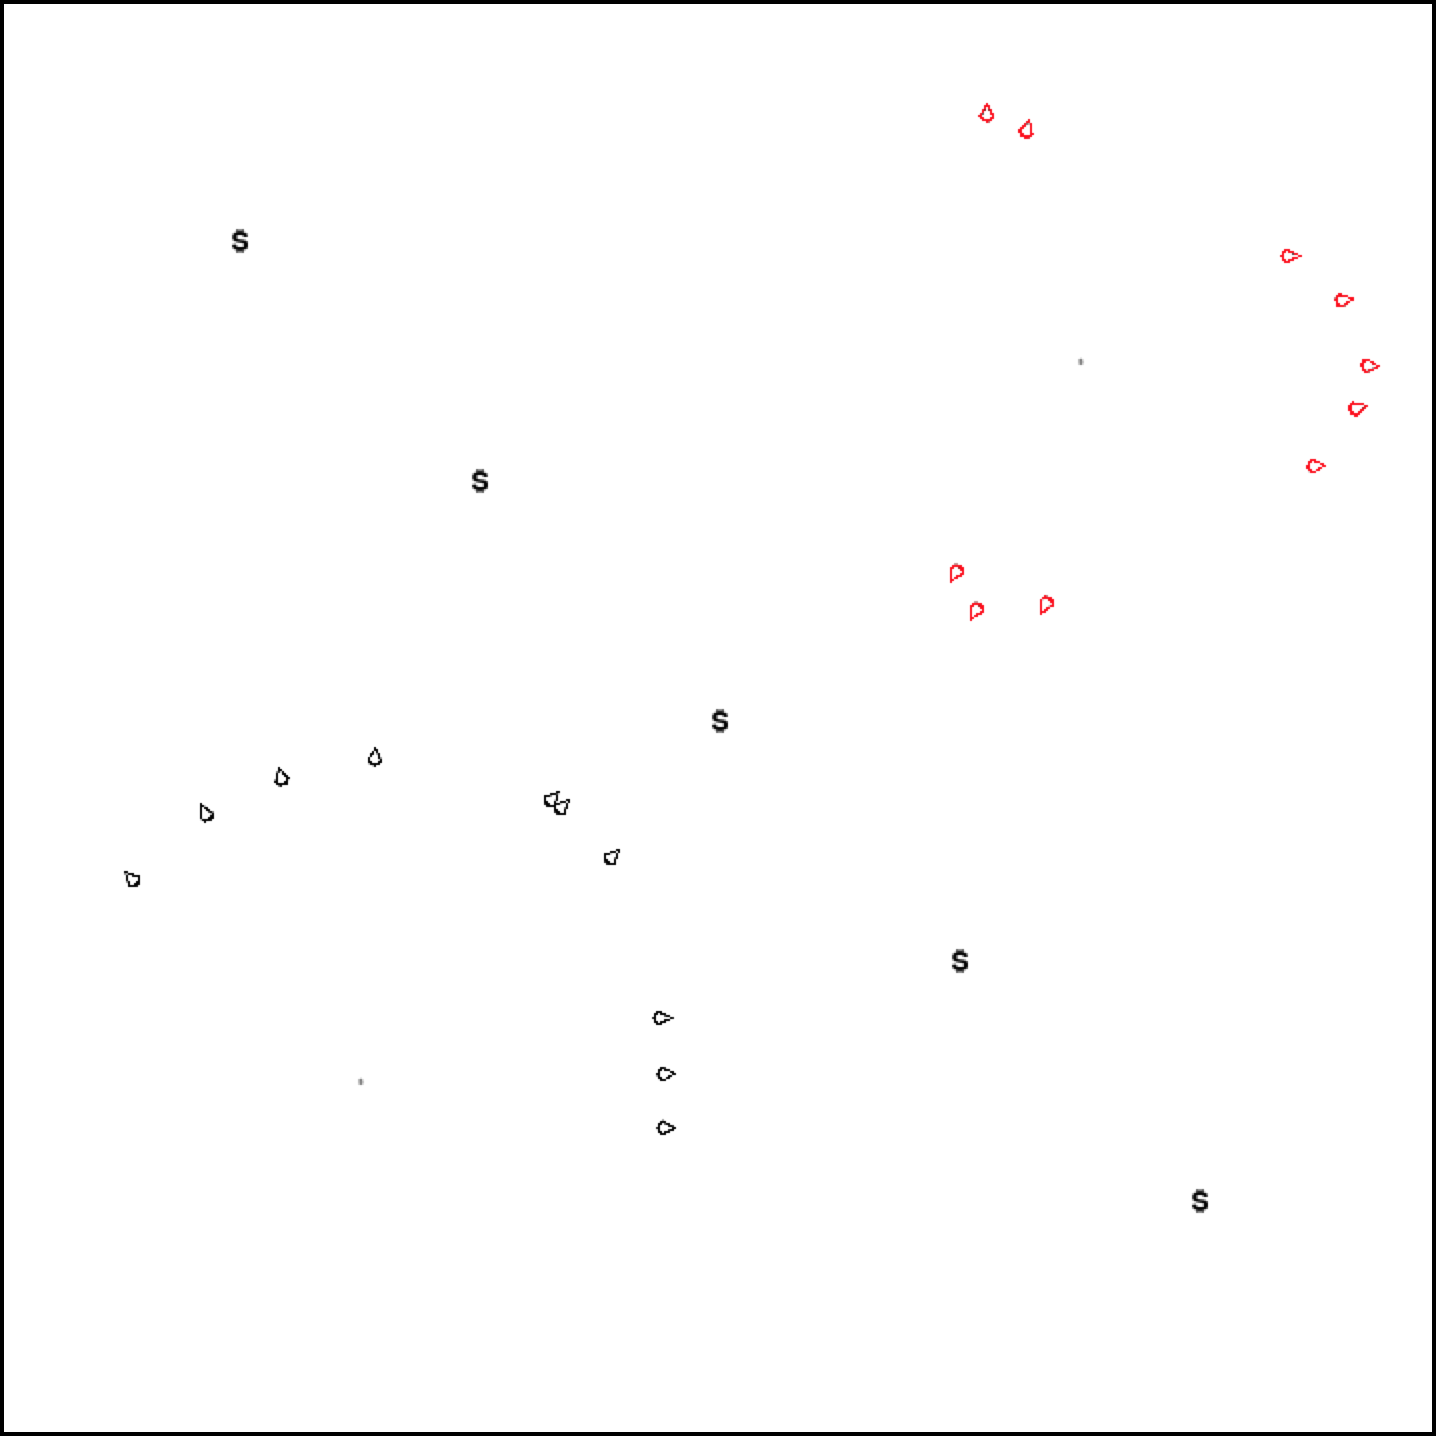
\includegraphics[width=0.5\textwidth]{figures/spreading}
    \caption{Screenshot of a visual simulation demonstrating two different types of spreading behavior for flocks that have differently designed movement behaviors.}
    \label{fig:spreading}
\end{figure}

However, the computational requirements for performing such an evolution is significant, particularly in terms of time. While parallel computation strategies enabled us to gather initial results, future work might include MapReduce implementations of the evolutionary computation to distribute tasks across a cluster of computers, as well as longer runs to ensure more significant evolutionary behavior. In order to carry out further experimentation at scale, some larger computational framework would be needed to implement the demands of the simulations. For example, potentially some other means of measuring fitness will be devised that are simulated faster, or a tiered simulation structure that first tests the team in isolation before running the simulation against an opposing team.

The work described in this paper represents only the first steps in the application of evolutionary techniques to the design of particles that exhibit flocking behavior. By mutating and applying selective pressure to the movement component parameters, we were able to show that a machine could optimize bottom-up velocity parameters better than a person, along with some limited state transition logic. However, because the states of the FSM controller were encoded in the simulation, we have not shown the ability to generate novel logical behaviors, but rather better collective strategies. A larger computational framework will hopefully allow us to dig deeper into our evolutionary mechanisms and refine them further.

Future work will also not ignore the Baldwin Effect, wherein machine learning techniques applied to the phenotypes will influence evolution by keeping genotypes that are able to learn around longer. Some phenotype learning system will also reduce the computational complexity of an evolutionary approach by itself. Additionally, other applications should be tested to show that evolutionary design of flocks performs well in many different simulated environments. For example, although the focus of our paper is on collective problem solving, we also see potential applications to improve optimization algorithms like PSO with movement rules that are evolved for particular optimization domains. PSO strategies could then be implemented that handle noise more effectively and particular swarms could be applied in selective conditions.

The next steps for this research would be to continue to evolve the structure of the FSM in more meaningful ways. In particular, new states should be generated by the configuration of individual velocity components as well as other evolved conditional rules, not just the state parameters. Of interest is the opportunity to evolve the transitions between states in a more significant manner, and then to go further and evolve the size and structure of the FSM by adding and removing states. One essential research question that should be answered is whether or not some form of crossover is possible in the FSM networks of particle swarms. If so, this will open up more opportunities for searching the optimal FSM space for collective movements. Other research questions might include better fitness functions that utilize the state of the entire world (for example, punishing swarms for allowing enemy agents to collect resources).

\IEEEtriggeratref{4}

\bibliographystyle{plain}
\bibliography{paper}

\end{document}
